\chapter{Radicais, carbenos e rearranjos}\label{ch:b3:radicals-carbenes}

O piretro, uma margarida, defende-se com ésteres do ácido crisantêmico, moléculas
construídas em torno de um anel de três carbonos; seus parentes sintéticos estão entre
os inseticidas domésticos mais usados. Os químicos fecham esses anéis em uma única etapa
adicionando um \omterm{def:b3:organometallic-bonding:carbene}{carbeno} a uma ligação dupla: um átomo de carbono com apenas seis elétrons
ao seu redor, dois deles não compartilhados. Este capítulo trata de intermediários reativos
que os volumes do 1.º e do 2.º ano só encontraram de passagem (os radicais usados em
síntese, os \omterm{def:b3:organometallic-bonding:carbene}{carbenos} e os \omterm{def:b3:radicals-carbenes:nitrene}{nitrenos}) e dos rearranjos nos quais um grupo
migra para um átomo de carbono, de nitrogênio ou de oxigênio deficiente em elétrons, entre eles dois
que produzem, a partir da mesma cetona, os monômeros do náilon-6 e de um poliéster biodegradável.

\begin{recall}
O volume do 1.º ano introduziu os radicais, a homólise e as setas de meia ponta,
os carbocátions e seus rearranjos, os nucleófilos e os grupos de saída; o
volume do 2.º ano, as cadeias radicalares (iniciação, propagação, terminação, iniciadores
radicalares), os perácidos, as lactonas, as lactamas e as iminas.
O \cref{ch:b3:complex-kinetics} tratou da cinética das \omterm{def:b3:complex-kinetics:chain}{reações em cadeia},
o \cref{ch:b3:organometallic-bonding}, dos \omterm{def:b3:organometallic-bonding:carbene}{carbenos} como ligantes,
o \cref{ch:b3:many-electron-atoms}, dos \omterm{def:b3:many-electron-atoms:singlet-triplet}{estados singleto} e tripleto, e
o \cref{ch:b3:rate-theories}, do postulado de Hammond.
\end{recall}

\begin{omfigure}
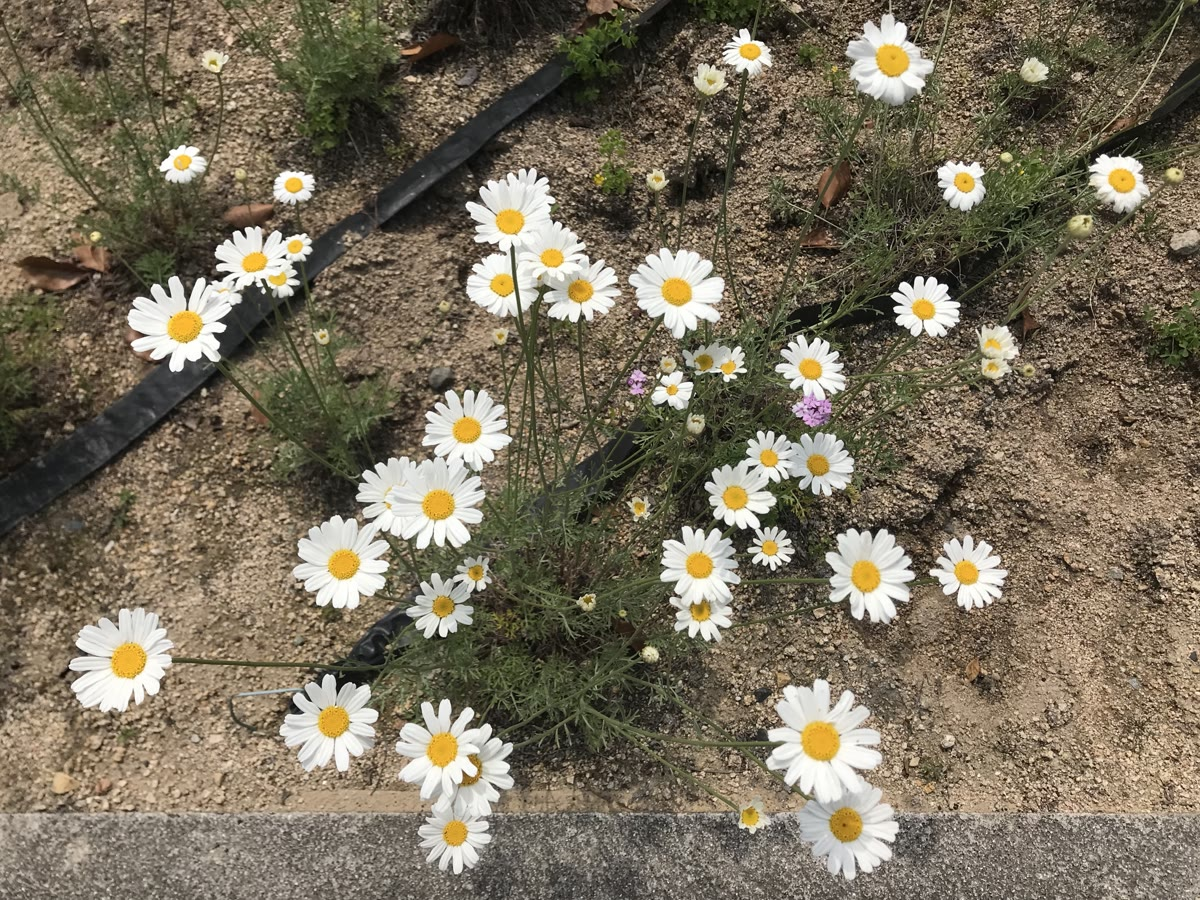
\includegraphics[width=0.48\linewidth]{images/book4/pyrethrum.jpg}

{\small Flores de piretro. Elas contêm as piretrinas, ésteres inseticidas
de um ácido ciclopropanocarboxílico. Fotografia: Soramimi, CC BY-SA 4.0.}
\end{omfigure}

\section{Reações radicalares em cadeia na síntese}

A estabilidade de um radical carbonado é medida pela entalpia de dissociação
da ligação C--H que o formaria: quanto mais fraca a ligação, mais
estável o radical.

\begin{proposition}[Entalpias de dissociação de ligação]\label{prop:b3:radicals-carbenes:bde}
A entalpia de dissociação da ligação R--H a \qty{298}{K} decorre das entalpias de formação
em fase gasosa: $\mathrm{BDE(R{-}H)} = \Delta_fH^\circ(\mathrm R^\bullet) + \Delta_fH^\circ(\mathrm H^\bullet) - \Delta_fH^\circ(\mathrm{RH})$.
\end{proposition}

\begin{proof}
A homólise $\mathrm{RH \to R^\bullet + H^\bullet}$ tem, pela lei de Hess, como entalpia de reação a de formação dos produtos
menos a do reagente; essa entalpia de reação é a entalpia de dissociação da ligação,
por definição.
\end{proof}

\begin{omfigure}
% ledger: dfh4:CH3r, dfh4:C2H5r, dfh4:iC3H7r, dfh4:tC4H9r, dfh4:PhCH2r, dfh4:H, dfh:CH4_g, dfh:C2H6_g, dfh:C3H8_g, dfh4:iC4H10, dfh4:toluene_g
\begin{tikzpicture}
\begin{axis}[width=0.72\linewidth, height=5.2cm, ybar, bar width=16pt, ymin=350, ymax=450,
  xtick={1,2,3,4,5}, xticklabels={{$\ce{CH3-H}$}, {$\ce{C2H5-H}$}, {$\mathrm{(CH_3)_2CH{-}H}$}, {$\mathrm{(CH_3)_3C{-}H}$}, {$\ce{C6H5CH2-H}$}},
  x tick label style={font=\scriptsize}, ylabel={BDE / \unit{kJ.mol^{-1}}},
  axis lines=left, tick label style={font=\scriptsize}, label style={font=\small},
  nodes near coords, nodes near coords style={font=\scriptsize, /pgf/number format/fixed, /pgf/number format/precision=0},
  enlarge x limits=0.15]
\addplot[fill=omDef!55, draw=omDef] table[x=i, y=bde] {figdata/out/bachelor-3-bde.dat};
\end{axis}
\end{tikzpicture}

{\small Entalpias de dissociação de ligações C--H a \qty{298}{K}, calculadas a partir das entalpias
de formação em fase gasosa das moléculas e dos radicais: metila, primário,
secundário, terciário e benzílico. A ligação enfraquece à medida que o radical formado é
mais substituído ou conjugado.}
\end{omfigure}

\begin{proposition}[Seletividade da halogenação]\label{prop:b3:radicals-carbenes:halogenation-selectivity}
A abstração de hidrogênio por um átomo de bromo é muito mais seletiva entre ligações C--H
primárias, secundárias e terciárias do que a abstração por um átomo de cloro.
\end{proposition}

\begin{proof}[Argumento]
Com $\mathrm{BDE(H{-}Cl)}$ maior que todos os valores C--H da figura e $\mathrm{BDE(H{-}Br)}$ menor,
a abstração pelo cloro é exotérmica e pelo bromo, endotérmica. Pelo postulado
de Hammond (\cref{ch:b3:rate-theories}), o estado de transição do cloro é precoce,
semelhante aos reagentes, e sente pouco a diferença entre os radicais formados;
o do bromo é tardio, semelhante aos produtos, e sua energia de ativação acompanha a maior parte
da diferença de BDE, que o fator de Boltzmann transforma em grandes razões de velocidade.
\end{proof}

O hidreto de tributilestanho reduz os haletos de alquila por uma cadeia: um radical de estanho toma o
halogênio, o radical alquila toma um átomo de hidrogênio da molécula seguinte de
hidreto, e forma-se um novo radical de estanho. A mesma cadeia remove um grupo hidróxi
depois que ele é transformado em um éster tiocarbonílico (a desoxigenação de
Barton--McCombie) e fecha anéis. Os resíduos organoestânicos são tóxicos e difíceis de
remover; o tris(trimetilsilil)silano e outros silanos substituem hoje com frequência o hidreto
de estanho.

\begin{omfigure}
\begin{tikzpicture}[font=\small, >=Stealth]
  \node (a) at (-2.0,0) {$\mathrm{Bu_3Sn^\bullet}$};
  \node (b) at (2.0,0) {$\mathrm{R^\bullet}$};
  \draw[->, thick] (a) to[bend left=35] node[midway, above, font=\scriptsize] {$+\,$R--Br, $\ -\,\mathrm{Bu_3SnBr}$} (b);
  \draw[->, thick] (b) to[bend left=35] node[midway, below, font=\scriptsize] {$+\,\mathrm{Bu_3SnH}$, $\ -\,$R--H} (a);
  \node[font=\scriptsize, align=center, anchor=north] at (0,-1.5) {iniciação: AIBN $\xrightarrow{\Delta}$ 2 R$'^\bullet$ $+$ $\ce{N2}$; \ R$'^\bullet$ $+$ $\mathrm{Bu_3SnH}$ $\to$ R$'$H $+$ $\mathrm{Bu_3Sn^\bullet}$};
\end{tikzpicture}

{\small As etapas de propagação de uma redução de um brometo de alquila por hidreto de estanho.
Cada R--Br reduzido consome um $\mathrm{Bu_3SnH}$ e dá um $\mathrm{Bu_3SnBr}$; os \omterm{def:b3:complex-kinetics:chain}{portadores de cadeia}
são o radical de estanho e o radical alquila.}
\end{omfigure}

O brometo de hidrogênio se adiciona aos alquenos pelo mesmo tipo de cadeia quando há
peróxidos presentes: um átomo de bromo se adiciona à extremidade menos substituída, dando o radical
mais estável, que toma então um átomo de hidrogênio do HBr: adição
anti-Markovnikov.

\section{Ciclizações radicalares}

\begin{definition}[Ciclizações exo e endo]\label{def:b3:radicals-carbenes:cyclisation}
Em uma \emph{ciclização exo}\index{ciclizacao exo@ciclização exo}, a ligação que se rompe (ou
a ligação $\pi$ atacada) fica fora do novo anel; em uma \emph{ciclização
endo}\index{ciclizacao endo@ciclização endo}, dentro dele.
\end{definition}

\begin{omfigure}
\begin{tikzpicture}[font=\scriptsize, >=Stealth]
  % hex-5-enyl radical: C1 radical, C5=C6
  \foreach \i/\a in {1/162, 2/234, 3/306, 4/18} { \coordinate (p\i) at (\a:0.9); }
  \coordinate (p5) at (90:0.95); \coordinate (p6) at (90:1.9);
  \draw[thick] (p1) -- (p2) -- (p3) -- (p4) -- (p5);
  \draw[thick, double, double distance=1.5pt] (p5) -- (p6);
  \node[anchor=east] at (p1) {$\bullet$\,1};
  \node[anchor=west] at (p5) {5}; \node[anchor=west] at (p6) {6};
  \draw[->, omMeth, thick] ($(p1)+(0.1,0.15)$) to[bend left=25] node[pos=0.45, below right, inner sep=1pt] {5-exo} ($(p5)+(-0.15,-0.05)$);
  \draw[->, omThm, thick, densely dashed] ($(p1)+(0,0.25)$) to[bend left=50] node[midway, left] {6-endo} ($(p6)+(-0.2,0)$);
  \node[font=\small, align=center] at (0,-1.6) {radical hex-5-enila};
  \draw[->, thick] (1.6,0.3) -- (2.7,0.3) node[midway, above] {rápida};
  \begin{scope}[xshift=4.0cm]
    \foreach \i/\a in {1/162, 2/234, 3/306, 4/18, 5/90} { \coordinate (q\i) at (\a:0.75); }
    \draw[thick] (q1) -- (q2) -- (q3) -- (q4) -- (q5) -- (q1);
    \draw[thick] (q5) -- ++(90:0.6) coordinate (q6);
    \node[anchor=south, inner sep=1pt] at (q6) {$\mathrm{{}^\bullet CH_2}$};
    \node[font=\small, align=center] at (0,-1.6) {radical ciclopentilmetila};
  \end{scope}
\end{tikzpicture}

{\small O radical 5-hexenila se fecha pelo ataque de C1 sobre C5 (5-exo, verde): o
novo anel tem cinco membros e o radical fica fora dele, em C6. O ataque sobre C6
(6-endo, tracejado vermelho) daria o radical ciclo-hexila secundário, mais estável,
mas é muito mais lento: a cadeia não consegue pôr C1 na linha de aproximação de C6 que
o orbital $\pi^*$ exige.}
\end{omfigure}

\begin{proposition}[Regras de Baldwin]\label{prop:b3:radicals-carbenes:baldwin}
Para os fechamentos de anel (estabelecidas experimentalmente, com uma justificativa
estereoeletrônica): em um carbono tetraédrico (tet), de 3- a 7-exo são favorecidos, 5- e
6-endo desfavorecidos; em um carbono trigonal (trig), de 3- a 7-exo são favorecidos, de 3- a 5-endo
desfavorecidos, 6- e 7-endo favorecidos; em um carbono digonal (dig), 3- e 4-exo são
desfavorecidos, de 5- a 7-exo favorecidos, de 3- a 7-endo favorecidos.
\end{proposition}

A justificativa é o ângulo de ataque que cada tipo de ligação exige: pela parte de trás da
ligação em um carbono tet, a cerca de 107° de um sistema $\pi$ trigonal, em um ângulo mais
fechado para uma ligação tripla; uma cadeia curta não consegue alcançar essas posições nos
casos desfavorecidos.

\begin{definition}[Relógio radicalar]\label{def:b3:radicals-carbenes:radical-clock}
Um \emph{relógio radicalar}\index{relogio radicalar@relógio radicalar} é um radical que se rearranja
de forma unimolecular com uma constante de velocidade conhecida, como o radical 5-hexenila
que se cicliza; sua competição com um captador bimolecular mede a constante de velocidade
do captador, ou o inverso.
\end{definition}

\begin{proposition}[Cinética de competição]\label{prop:b3:radicals-carbenes:clock}
Se um radical ou se cicliza ($k_c$) ou é capturado por um hidreto mantido em excesso na
concentração $[\mathrm{R_3SnH}]$ ($k_H$), a razão dos produtos é
$[\text{ciclizado}]/[\text{direto}] = k_c/(k_H[\mathrm{R_3SnH}])$.
\end{proposition}

\begin{proof}
A cada instante, os dois produtos se formam com velocidades $k_c[\mathrm R^\bullet]$ e $k_H[\mathrm{R_3SnH}][\mathrm R^\bullet]$. Sua razão
não depende da concentração de radical, que varia; com a concentração de hidreto
constante, a integração no tempo multiplica ambas pela mesma
$\int[\mathrm R^\bullet]\,\dd t$, e a razão dos produtos é a razão das constantes de velocidade
vezes $1/[\mathrm{R_3SnH}]$.
\end{proof}

\begin{omfigure}
\begin{tikzpicture}
\begin{axis}[name=a, width=0.47\linewidth, height=5.2cm, xmode=log, xmin=1e-3, xmax=1, ymin=0, ymax=1,
  axis lines=left, xlabel={$[\mathrm{Bu_3SnH}]$ / \unit{mol.L^{-1}}}, ylabel={fração ciclizada},
  tick label style={font=\scriptsize}, label style={font=\small}]
\addplot[omDef, thick] table[x=c, y=fcyc] {figdata/out/bachelor-3-radical-clock.dat};
\end{axis}
\begin{axis}[at={(a.east)}, anchor=west, xshift=1.5cm, width=0.47\linewidth, height=5.2cm,
  xmin=0, xmax=1, ymin=0, ymax=11, axis lines=left,
  xlabel={$[\mathrm{Bu_3SnH}]$ / \unit{mol.L^{-1}}}, ylabel={[direto]/[ciclizado]},
  tick label style={font=\scriptsize}, label style={font=\small}]
\addplot[omThm, thick] table[x=c, y=inv] {figdata/out/bachelor-3-radical-clock-b.dat};
\node[font=\scriptsize, anchor=west, omThm] at (axis cs:0.15,7.5) {inclinação $k_H/k_c$};
\end{axis}
\end{tikzpicture}

{\small O relógio 5-hexenila com as constantes de velocidade do modelo $k_c = \qty{2.3e5}{s^{-1}}$ e
$k_H = \qty{2.4e6}{L.mol^{-1}.s^{-1}}$. À esquerda: fração de metilciclopentano entre os produtos em função da
concentração de hidreto: metade em $k_c/k_H \approx \qty{0.1}{mol/L}$. À direita: a razão inversa é uma reta
que passa pela origem, de inclinação $k_H/k_c$.}
\end{omfigure}

\begin{method}[Planejar uma redução ou uma ciclização radicalar]\label{met:b3:radicals-carbenes:radical-chain}
\begin{enumerate}
  \item Para uma redução simples, mantenha o doador de hidrogênio concentrado (cerca de
        \qty{0.1}{mol/L} ou mais), de modo que o radical seja capturado antes de se rearranjar.
  \item Para uma ciclização, mantenha o doador diluído, ou adicione-o lentamente, de modo que o
        radical se ciclize primeiro: escolha $[\text{doador}] \ll k_c/k_H$.
  \item Escolha um iniciador cuja meia-vida à temperatura da reação seja da
        ordem do tempo de reação (AIBN perto de \qty{80}{\celsius}) e adicione-o em porções, se
        necessário.
  \item Prefira um silano ou outro doador sem estanho, e remova o oxigênio, que captura
        os radicais carbonados.
\end{enumerate}
\end{method}

\begin{inthelab}[Adição lenta com bomba de seringa]
Para manter um reagente diluído durante toda uma reação, sua solução é carregada em uma
seringa estanque a gases e adicionada através de um septo por uma bomba de seringa ao longo de várias
horas, na solução do substrato a refluxo, sob nitrogênio. A
concentração do reagente permanece então perto de seu baixo valor estacionário, fixado pela
velocidade de adição e pela velocidade com que ele é consumido.
\end{inthelab}

\section{Carbenos}

\begin{definition}[Carbenos singleto e tripleto]\label{def:b3:radicals-carbenes:carbene-states}
Um \emph{carbeno singleto}\index{carbeno singleto} tem seus dois elétrons não ligantes
emparelhados em um orbital, um híbrido $sp^2$, com seu orbital p vazio; um
\emph{carbeno tripleto}\index{carbeno tripleto} os tem desemparelhados, um em cada
orbital, com spins paralelos.
\end{definition}

\begin{omfigure}
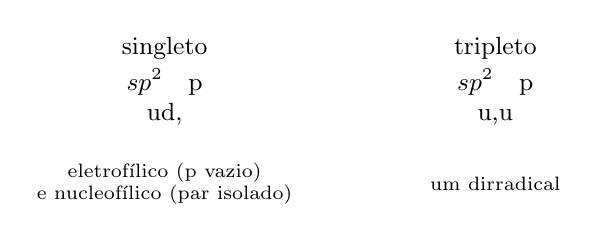
\begin{tikzpicture}[font=\small]
  \node[align=center] at (0,0) {singleto\\[2pt] $sp^2$ \ \ p\\ \omorbs{ud,}};
  \node[align=center] at (4.2,0) {tripleto\\[2pt] $sp^2$ \ \ p\\ \omorbs{u,u}};
  \node[font=\scriptsize, align=center] at (0,-1.3) {eletrofílico (p vazio)\\ e nucleofílico (par isolado)};
  \node[font=\scriptsize, align=center] at (4.2,-1.3) {um dirradical};
\end{tikzpicture}

{\small Ocupação eletrônica dos dois orbitais não ligantes de um \omterm{def:b3:organometallic-bonding:carbene}{carbeno}. O
tripleto é o estado fundamental do $\ce{CH2}$; os substituintes $\pi$-doadores (Cl, OR, $\mathrm{NR_2}$) elevam o
orbital p e fazem do singleto o estado fundamental, como no diclorocarbeno.}
\end{omfigure}

Os \omterm{def:b3:organometallic-bonding:carbene}{carbenos} são preparados pela perda de dinitrogênio de um composto diazo (por calor, luz
ou um catalisador metálico), por $\alpha$-eliminação (o clorofórmio e uma base forte dão
$\ce{CCl3-}$, que perde cloreto dando $\ce{CCl2}$), ou são totalmente evitados por meio de um
\omterm{def:b3:radicals-carbenes:carbenoid}{carbenoide}.

\begin{definition}[Carbenoides]\label{def:b3:radicals-carbenes:carbenoid}
Um \emph{carbenoide}\index{carbenoide} é uma espécie ligada a um metal que transfere um
grupo \omterm{def:b3:organometallic-bonding:carbene}{carbeno} como um \omterm{def:b3:organometallic-bonding:carbene}{carbeno} livre o faria, sem que o \omterm{def:b3:organometallic-bonding:carbene}{carbeno} livre se forme,
como o iodeto de iodometilzinco $\ce{ICH2ZnI}$ da reação de Simmons--Smith.
\end{definition}

\begin{definition}[Ciclopropanação]\label{def:b3:radicals-carbenes:cyclopropanation}
A \emph{ciclopropanação}\index{ciclopropanacao@ciclopropanação} é a formação de um
ciclopropano pela adição de um \omterm{def:b3:organometallic-bonding:carbene}{carbeno} ou de um \omterm{def:b3:radicals-carbenes:carbenoid}{carbenoide} a uma ligação dupla C=C.
\end{definition}

\begin{proposition}[O teste de Skell]\label{prop:b3:radicals-carbenes:skell}
Um \omterm{def:b3:radicals-carbenes:carbene-states}{carbeno singleto} se adiciona a um alqueno \textit{cis} ou \textit{trans} de modo estereoespecífico, conservando a
configuração relativa; um \omterm{def:b3:radicals-carbenes:carbene-states}{carbeno tripleto} dá os dois estereoisômeros do
ciclopropano.
\end{proposition}

\begin{proof}[Argumento]
O singleto forma as duas novas ligações em uma única etapa concertada, sem tempo para
rotação. O tripleto forma primeiro uma ligação, dando um 1,3-dirradical tripleto; seus
dois elétrons desemparelhados não podem formar a segunda ligação até que um spin se inverta, o que é
lento em comparação com a rotação em torno da ligação simples C--C restante: a
configuração se embaralha.
\end{proof}

\begin{omfigure}
\setchemfig{atom sep=1.8em}
\schemestart
\chemfig{H_3C-[:30]=[:0]-[:-30]CH_3}
\arrow{->[singleto $\ce{CH2}$]}[,1.6]
\chemfig{(<[:210]H_3C)-[:0](<[:330]CH_3)-[:120]-[:240]}
\schemestop
\par\medskip

{\small Teste de Skell: o \textit{cis}-but-2-eno, com os dois grupos metila do mesmo lado, dá com
um \omterm{def:b3:radicals-carbenes:carbene-states}{carbeno singleto} apenas o \textit{cis}-1,2-dimetilciclopropano (os dois grupos metila em cunhas,
na mesma face do anel); com um \omterm{def:b3:radicals-carbenes:carbene-states}{carbeno
tripleto}, aparece também o isômero \textit{trans}.}
\end{omfigure}

Os \omterm{def:b3:radicals-carbenes:carbene-states}{carbenos singleto} também se inserem em ligações C--H. Os carboxilatos de ródio(II)
decompõem os diazoésteres em \omterm{def:b3:radicals-carbenes:carbenoid}{carbenoides} de ródio que ciclopropanam alquenos e
se inserem em ligações C--H de modo seletivo e, com ligantes quirais, enantiosseletivo.

\begin{definition}[Nitrenos]\label{def:b3:radicals-carbenes:nitrene}
Um \emph{nitreno}\index{nitreno} $\mathrm{R{-}\ddot N}$ é o análogo nitrogenado de um \omterm{def:b3:organometallic-bonding:carbene}{carbeno}, um átomo de
nitrogênio neutro com apenas seis elétrons, formado, por exemplo, pela perda de
dinitrogênio de uma azida.
\end{definition}

\section{Rearranjos para um carbono deficiente em elétrons}

\begin{definition}[Deslocamento 1,2]\label{def:b3:radicals-carbenes:shift}
Um \emph{deslocamento 1,2}\index{deslocamento 1,2} é a migração de um grupo, com seu par
ligante, de um átomo para o átomo vizinho deficiente em elétrons.
\end{definition}

Em um deslocamento de Wagner--Meerwein, um grupo alquila ou um hidreto passa para um carbocátion
vizinho, dando um mais estável: os rearranjos de carbocátions do
volume do 1.º ano, agora com seu mecanismo nomeado. Os esqueletos dos terpenos são remodelados
na natureza por cascatas desses deslocamentos.

\begin{definition}[Rearranjo pinacólico]\label{def:b3:radicals-carbenes:pinacol}
O \emph{rearranjo pinacólico}\index{rearranjo pinacolico@rearranjo pinacólico} transforma um 1,2-diol,
em meio ácido, em uma cetona ou em um aldeído: um grupo hidróxi sai como água, um
grupo do carbono vizinho se desloca para o cátion, e o cátion formado,
estabilizado pelo oxigênio restante, perde um próton.
\end{definition}

\begin{definition}[Aptidão migratória]\label{def:b3:radicals-carbenes:migratory}
A \emph{aptidão migratória}\index{aptidao migratoria@aptidão migratória} de um grupo é sua
tendência relativa a migrar em um \omterm{def:b3:radicals-carbenes:shift}{deslocamento 1,2} para um centro deficiente em elétrons.
\end{definition}

Os grupos que suportam bem uma carga positiva durante o deslocamento migram melhor: hidreto,
arila e alquila terciária antes da secundária, da primária e da metila. Assim, o pinacol,
$\mathrm{(CH_3)_2C(OH){-}C(OH)(CH_3)_2}$, dá a pinacolona, 3,3-dimetilbutan-2-ona.

\begin{method}[Prever o produto de um rearranjo]\label{met:b3:radicals-carbenes:rearrangement}
\begin{enumerate}
  \item Encontre o átomo deficiente em elétrons formado (cátion, nitrênio, oxigênio de um
        peróxido ativado, \omterm{def:b3:organometallic-bonding:carbene}{carbeno} ou \omterm{def:b3:radicals-carbenes:nitrene}{nitreno}) e o grupo de saída que o cria.
  \item Liste os grupos do átomo vizinho que poderiam migrar; quando a
        geometria é fixa (oximas), só pode migrar o grupo anti ao grupo de saída.
  \item Caso contrário, escolha pela \omterm{def:b3:radicals-carbenes:migratory}{aptidão migratória}, ou pelo grupo que forma o cátion mais
        estável no ponto de onde sai.
  \item Desloque o grupo com retenção de sua configuração, depois complete o
        mecanismo (perda de um próton, adição de água).
\end{enumerate}
\end{method}

\section{Rearranjos para um nitrogênio ou um oxigênio deficiente em elétrons}

\begin{definition}[Rearranjo de Beckmann]\label{def:b3:radicals-carbenes:beckmann}
O \emph{rearranjo de Beckmann}\index{rearranjo de Beckmann} transforma uma oxima,
em ácido forte, em uma amida: o grupo hidróxi, ativado como grupo de saída,
parte enquanto o grupo anti a ele migra do carbono para o nitrogênio; a água se adiciona
ao íon nitrílio formado, e a tautomerização dá a amida.
\end{definition}

\begin{proposition}[Migração anti]\label{prop:b3:radicals-carbenes:beckmann-anti}
No \omterm{def:b3:radicals-carbenes:beckmann}{rearranjo de Beckmann}, o grupo que migra é o que está em anti em relação ao
grupo de saída no nitrogênio.
\end{proposition}

\begin{proof}[Argumento]
O par da ligação que migra ataca o nitrogênio pela parte de trás da ligação N--O, como em um
deslocamento $\mathrm S_\mathrm N2$; só o grupo anti ao oxigênio tem sua ligação alinhada com
o orbital $\sigma^*$ N--O. A etapa é concertada com a saída do grupo de saída,
de modo que não se forma nenhum íon nitrênio livre que pudesse escolher de outra forma.
\end{proof}

\begin{omfigure}
\setchemfig{atom sep=1.9em}
\schemestart
\chemfig{*6(-----(=N-[:30]OH)-)}
\arrow{->[$\ce{H2SO4}$ (óleum)][Beckmann]}[,1.8]
\chemfig{*7(---N(-[:-90]H)-(=O)---)}
\schemestop
\par\medskip
\schemestart
\chemfig{*6(-----(=O)-)}
\arrow{->[perácido][Baeyer--Villiger]}[,1.8]
\chemfig{*7(-----O-(=O)-)}
\schemestop

{\small Duas expansões de anel da ciclo-hexanona. Acima: sua oxima se rearranja no
óleum em caprolactama (azepan-2-ona), o monômero do náilon-6, com o nitrogênio entrando
no anel. Abaixo: um perácido insere um átomo de oxigênio ao lado do grupo
carbonila, dando a $\varepsilon$-caprolactona (oxepan-2-ona).}
\end{omfigure}

\begin{definition}[Oxidação de Baeyer--Villiger]\label{def:b3:radicals-carbenes:baeyer}
A \emph{oxidação de Baeyer--Villiger}\index{oxidacao de Baeyer--Villiger@oxidação de Baeyer--Villiger} transforma uma
cetona em um éster, ou uma cetona cíclica em uma lactona, com um perácido: o
perácido se adiciona ao grupo carbonila, depois um grupo do carbono carbonílico
migra para o oxigênio peroxídico mais próximo enquanto um carboxilato sai.
\end{definition}

\begin{proposition}[Regioquímica de Baeyer--Villiger]\label{prop:b3:radicals-carbenes:bv-retention}
Na \omterm{def:b3:radicals-carbenes:baeyer}{oxidação de Baeyer--Villiger}, o grupo que migra conserva sua
configuração, e a ordem de \omterm{def:b3:radicals-carbenes:migratory}{aptidão migratória} é alquila terciária >
alquila secundária $\approx$ arila > alquila primária > metila (estabelecida experimentalmente).
\end{proposition}

\begin{proof}[Argumento]
O grupo se desloca com seu par ligante pela face do carbono que deixa
e chega ao oxigênio pelo mesmo lado, de modo que sua configuração se conserva. No
estado de transição, o grupo que migra carrega uma carga positiva parcial, que a
substituição alquila e a conjugação arila estabilizam.
\end{proof}

\begin{definition}[Isocianatos, rearranjos de Curtius e de Hofmann]\label{def:b3:radicals-carbenes:curtius}
Um \emph{isocianato}\index{isocianato} é um composto $\ce{R-N=C=O}$. No \emph{rearranjo de Curtius}%
\index{rearranjo de Curtius}, uma acilazida perde dinitrogênio por
aquecimento enquanto o grupo R passa do carbono para o nitrogênio, dando um isocianato;
no \emph{rearranjo de Hofmann}\index{rearranjo de Hofmann}, uma amida primária
tratada com bromo e base dá o mesmo isocianato por meio de uma
N-bromoamida. Com a água, o isocianato dá a amina $\ce{RNH2}$ e dióxido de
carbono; com um álcool, um carbamato.
\end{definition}

\begin{definition}[Cetenas e o rearranjo de Wolff]\label{def:b3:radicals-carbenes:wolff}
Uma \emph{cetena}\index{cetena} é um composto $\mathrm{R_2C{=}C{=}O}$. No \emph{rearranjo de Wolff}%
\index{rearranjo de Wolff}, uma $\alpha$-diazocetona perde dinitrogênio
enquanto o grupo do carbono carbonílico migra, dando uma cetena, que adiciona
água, um álcool ou uma amina.
\end{definition}

O \omterm{def:b3:radicals-carbenes:wolff}{rearranjo de Wolff} é a etapa-chave da homologação de Arndt--Eistert,
que alonga um ácido carboxílico em um carbono: cloreto de ácido, depois
diazocetona, depois \omterm{def:b3:radicals-carbenes:wolff}{cetena}, depois o ácido homólogo.

\begin{safety}{\ghs[0.62cm]{GHS06}\ghs[0.62cm]{GHS08}\ghs[0.62cm]{GHS09}}
% ledger: ghs4:Bu3SnH, ghs4:diazomethane, ghs4:AIBN
Hidreto de tributilestanho: tóxico se ingerido, nocivo em contato com a pele, provoca danos aos órgãos por
exposição repetida, muito tóxico para os organismos aquáticos; os resíduos de estanho são recolhidos
separadamente. O diazometano é um gás tóxico, cancerígeno e explosivo; ele é
citado aqui apenas por sua química e é substituído na prática por reagentes mais seguros,
como o trimetilsilildiazometano. O AIBN é autorreativo por aquecimento.
\end{safety}

\begin{history}[Um radical que não deveria existir, e um náilon]
Em 1900, Moses Gomberg, tentando preparar o hexafeniletano, obteve uma solução amarela
que absorvia oxigênio e iodo: o radical trifenilmetila, o primeiro
radical carbonado persistente. Meio século depois, o \omterm{def:b3:radicals-carbenes:beckmann}{rearranjo de Beckmann} da
oxima da ciclo-hexanona tornou-se a rota industrial para a caprolactama, polimerizada por
abertura de anel em náilon-6, uma fibra e um plástico de engenharia produzidos em escala
muito grande.
\end{history}

\section{Exercícios}

\begin{exercise}[$\star$]\label{exo:b3:radicals-carbenes:1}
A \qty{25}{\celsius}, as reatividades relativas por hidrogênio das ligações C--H primárias, secundárias e
terciárias são $1 : 3.9 : 5.1$ frente aos átomos de cloro e $1 : 82 : 1600$ frente aos
átomos de bromo (dados do exercício). Calcule as proporções de 1- e de 2-halopropano
formadas a partir do propano em cada caso.
\end{exercise}

\begin{exercise}[$\star$]\label{exo:b3:radicals-carbenes:2}
Qual é o estado fundamental do $\ce{CH2}$, e do $\ce{CCl2}$? Qual deles se adiciona de modo estereoespecífico ao
\textit{trans}-but-2-eno, e o que ele dá?
\end{exercise}

\begin{exercise}[$\star$]\label{exo:b3:radicals-carbenes:3}
Dê o produto da reação de Simmons--Smith do (\textit{Z})-hex-3-eno.
\end{exercise}

\begin{exercise}[$\star$]\label{exo:b3:radicals-carbenes:4}
Dê os produtos da \omterm{def:b3:radicals-carbenes:baeyer}{oxidação de Baeyer--Villiger} da ciclo-hexanona e da
acetofenona.
\end{exercise}

\begin{exercise}[$\star\star$]\label{exo:b3:radicals-carbenes:5}
Com os dados do \cref{exo:b3:radicals-carbenes:1}, calcule as proporções dos
dois monocloretos e dos dois monobrometos do 2-metilpropano.
\end{exercise}

\begin{exercise}[$\star\star$]\label{exo:b3:radicals-carbenes:6}
Um novo \omterm{def:b3:radicals-carbenes:radical-clock}{relógio radicalar}, reduzido com $\qty{0.020}{mol/L}$ de $\mathrm{Bu_3SnH}$, dá três vezes mais produto rearranjado
que não rearranjado. Com $k_H = \qty{2.4e6}{L.mol^{-1}.s^{-1}}$, encontre sua constante de velocidade.
\end{exercise}

\begin{exercise}[$\star\star$]\label{exo:b3:radicals-carbenes:7}
Classifique pelas regras de Baldwin o ataque de um radical hex-5-enila sobre C5 e sobre C6,
depois diga se cada um destes fechamentos é favorecido: 4-exo-tet, 5-endo-trig,
5-exo-dig, 3-exo-dig, 5-endo-dig.
\end{exercise}

\begin{exercise}[$\star\star$]\label{exo:b3:radicals-carbenes:8}
Dê o produto do \omterm{def:b3:radicals-carbenes:pinacol}{rearranjo pinacólico} do 2,3-difenilbutano-2,3-diol
e explique a escolha do grupo que migra.
\end{exercise}

\begin{exercise}[$\star\star$]\label{exo:b3:radicals-carbenes:9}
A azida de benzoíla é aquecida em tolueno e depois se adiciona água; em um segundo experimento,
etanol. Dê os produtos.
\end{exercise}

\begin{exercise}[$\star\star\star$]\label{exo:b3:radicals-carbenes:10}
Com $\mathrm{BDE(H{-}Cl)} = \qty{432}{kJ/mol}$ e $\mathrm{BDE(H{-}Br)} = \qty{366}{kJ/mol}$ (dados do exercício) e os valores C--H da
figura do capítulo, calcule $\Delta H$ da abstração de um hidrogênio primário e de um terciário
por cada átomo de halogênio, e use o postulado de Hammond para explicar as
seletividades do \cref{exo:b3:radicals-carbenes:1}.
\end{exercise}

\begin{exercise}[$\star\star\star$]\label{exo:b3:radicals-carbenes:11}
Dê os produtos de Beckmann das duas oximas, \textit{E} e \textit{Z}, da 2-metilciclo-hexanona,
e explique por que eles diferem, enquanto a \omterm{def:b3:radicals-carbenes:baeyer}{oxidação de Baeyer--Villiger} da
cetona dá uma única lactona principal.
\end{exercise}

\begin{exercise}[$\star\star\star$]\label{exo:b3:radicals-carbenes:12}
Com o relógio-modelo do capítulo, calcule a fração ciclizada para $[\mathrm{Bu_3SnH}] = 0.010$,
0.10 e \qty{1.0}{mol/L}. Que concentração de hidreto dá 95\,\% de produto ciclizado, e como
ela pode ser mantida?
\end{exercise}

\section{Problema: Dois anéis a partir da ciclo-hexanona}

\begin{problem}[{Problema de fim de semana --- dois anéis a partir da ciclo-hexanona: a oxima, o
rearranjo de Beckmann em caprolactama, a oxidação de Baeyer--Villiger em
caprolactona e a regioquímica das duas com a 2-metilciclo-hexanona}]
\label{pb:b3:radicals-carbenes:1}
% ledger: aw:C, aw:H, aw:N, aw:O, aw:S
Dados do problema: uma tonelada de ciclo-hexanona é convertida em sua oxima com
98\,\% de rendimento, e a oxima em caprolactama com 98\,\% de rendimento; o rearranjo usa
1.3 mol de ácido sulfúrico (na forma de óleum) por mol de oxima, neutralizado no fim com
amônia, dando sulfato de amônio.

\medskip\noindent\textbf{Parte I --- A oxima.}
\begin{enumerate}
  \item Escreva a formação da oxima da ciclo-hexanona a partir da hidroxilamina.
  \item Por que ela é realizada perto de pH 4 a 5?
  \item A oxima da ciclo-hexanona tem isômeros \textit{E} e \textit{Z}? Por quê?
  \item Desenhe as oximas \textit{E} e \textit{Z} da 2-metilciclo-hexanona.
  \item Por que essas duas oximas só se interconvertem lentamente?
\end{enumerate}

\medskip\noindent\textbf{Parte II --- O \omterm{def:b3:radicals-carbenes:beckmann}{rearranjo de Beckmann}.}
\begin{enumerate}[resume]
  \item O que o ácido faz com a oxima?
  \item Que ligação migra, e por que ela torna o anel maior?
  \item Que intermediário a água ataca?
  \item Escreva a equação global, da oxima à caprolactama.
  \item Nomeie e desenhe o produto, e o polímero obtido a partir dele.
  \item Calcule as massas molares da ciclo-hexanona e da caprolactama.
  \item Calcule a massa de caprolactama obtida a partir de uma tonelada de ciclo-hexanona.
  \item Calcule a massa de sulfato de amônio produzida junto com ela.
\end{enumerate}

\medskip\noindent\textbf{Parte III --- A \omterm{def:b3:radicals-carbenes:baeyer}{oxidação de Baeyer--Villiger}.}
\begin{enumerate}[resume]
  \item Escreva a oxidação da ciclo-hexanona por um perácido $\ce{RCO3H}$.
  \item Dê o intermediário formado pela adição do perácido.
  \item Que grupo migra, e qual é o grupo de saída?
  \item Nomeie a lactona e o polímero que ela dá.
  \item Por que o peróxido de hidrogênio com um catalisador pode substituir o perácido em um
        processo mais limpo?
\end{enumerate}

\medskip\noindent\textbf{Parte IV --- A 2-metilciclo-hexanona.}
\begin{enumerate}[resume]
  \item Que carbono migra em sua \omterm{def:b3:radicals-carbenes:baeyer}{oxidação de Baeyer--Villiger}, e que lactona se forma?
  \item A configuração desse carbono se conserva?
  \item Que lactama a oxima \textit{E} dá (OH anti ao carbono que porta a metila)?
  \item Que lactama a oxima \textit{Z} dá?
  \item O que decide a regioquímica em cada reação?
  \item Por que a própria ciclo-hexanona está livre desses problemas?
  \item Enuncie o resultado: a massa de caprolactama obtida a partir de uma tonelada de ciclo-hexanona.
\end{enumerate}
\end{problem}
